\section{Resultados}

En la tabla \ref{tab:scores} podemos observar los resultados obtenidos por el clasificador. Se midieron la efectividad (accuracy), precisión, exactitud (recall) y área bajo la curva ROC. 

\begin{table}[t]
    \centering
    \begin{tabular}{|c|c|c|c|c|}
        \hline
        Clasificador & Accuracy & Precision & Recall & ROC AUC  \\\hline
        CNN-1 & 0.55 & 0.21 & 0.65 & 0.64 \\
        CNN-2 & 0.59 & 0.23 & 0.61 & 0.64 \\
        CNN-3 & 0.52 & 0.22 & 0.72 & 0.66 \\
        \hline 
    \end{tabular}
    \caption{Resultados de la clasificación}
    \label{tab:scores}
\end{table}

A su vez, por la topología planteada, es posible analizar los filtros obtenidos en la primer capa. Estos representan combinaciones de electrodos que resultaron del entrenamiento de la red. En la figura \ref{fig:kernels} se pueden apreciar los pesos obtenidos para algunos de los filtros entrenados


\begin{figure}
    \centering
    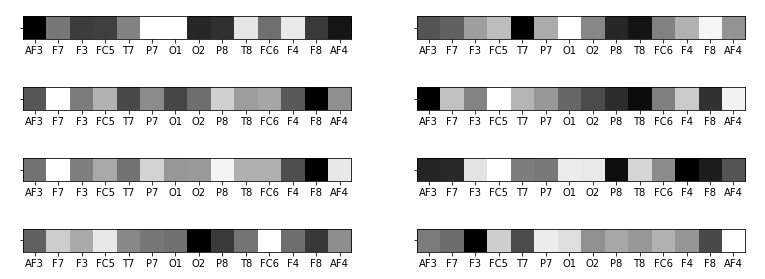
\includegraphics[scale=0.5]{channel_filters.png}
    \caption{Filtros espaciales obtenidos. Más oscuro implica más peso}
    \label{fig:kernels}
\end{figure}


\section{Discusión y trabajo a futuro}

Los resultados obtenidos en este trabajo se asemejan a los de \cite{cecotti2011}; sin embargo, es de notar que nuestros datos son de calidad sensiblemente menor ya que fueron tomados por equipamiento con mucha menor resolución espacial y temporal. A su vez, las condiciones de recolección de los datos son mucho más ruidosas.

Sin embargo, los resultados son interesantes ya que pueden permitirnos pre-entrenar una red neuronal profunda para detectar P300 con alta precisión, ajustando las capas finales de acuerdo a cada usuario.

Como trabajo a futuro, nos queda analizar un poco mejor los datos para sacar aquellos muy ruidosos, refinar datos haciendo una selección de los mejores electrodos. A su vez, queda efectuar la detección del caracter, que es la tarea usualmente medida en esta aplicación de BCI.